\documentclass[12pt,fleqn]{article}\usepackage{../../common}
\begin{document}
Paralel Lineer Cebir Temeli

[5] adlı yazı tek makinalı ortamda matris çarpımının nasıl yapılacağını, ve
nasıl görülecebileğini anlattı. Satır bakış açısı, kolon bakış açısı
işlendi. Parallel (Hadoop), eşle/indirge ortamında matris çarpımını nasıl
yaparız?  Mesela $A^TA$'yi ele alalım. Bu çarpım oldukça önemli çünkü başka
sonuçlar için de kullanılabiliyor. Mesela $A$ üzerinde $QR$ ayrıştırması
yapmak isterseniz (bkz. Lineer Cebir ders notlarımız) bu çarpım
kullanılabiliyor.

Nasıl? QR ayrıştırması kolonların hepsi bilindiği gibi birbirine dik
(orthogonal) birim vektörler olan bir $Q$ matrisi ve üst üçgensel (upper
triangular) bir $R$ matrisi oluşturur. Ayrıştırmanın $A^TA$ ile bağlantısı
nedir? Eğer $A$ yerine onun ayrıştırmasını $QR$ koyarsak,

$$
C = A^TA = (QR)^T (QR) = R^T Q^T QR
$$

Tum $Q$ vektorleri birbirine dik, ve birim vektorler ise, $Q^T Q$
birim matrisi $I$ olur. O zaman

$$
C = R^T Q^T QR = R^T R
$$

Yani

$$
C = R^TR
$$

Peki $A^TA$ hesaplayıp (böylece $R^TR$'yi elde edince) onun içinden $R$'yi nasıl
çekip çıkartırız? Şimdi Cholesky ayrıştırması kullanmanın zamanı. Cholesky
ayrıştırması (herhangi bir simetrik pozitif kesin $C$ matrisi üzerinde)

$$C = LL^T$$

olarak bilinir, yani bir matris alt üçgensel (lower triangular -ki L harfi
oradan geliyor-) $L$ matrisine ve onun devriği olan üst üçgensel $L^T$'nin
çarpımına ayrıştırılır. Elimizde $R^TR$ var, ve ona benzer $LL^T$ var, $R$
bilindiği gibi üst üçgensel, $L$ alt üçgensel, $L^T$ ve $R$ birbirine eşit demek
ki. Yani $A^TA$ üzerinde sayısal hesap kütüphenimzin Cholesky çağrısı kullanmak
bize $QR$'in $R$'sini verir.

Şu anda akla şu soru gelebilir: madem kütüphane çağrısı yaptık, niye $A$
üzerinde kütüphenimizin $QR$ çağrısını kullanmıyoruz?

Cevap Büyük Veri argümanında saklı. Bu ortamda uğraşılan verilerde $A$ matrisi
$m \times n$ boyutlarındadır, ve $m$ milyonlar, hatta milyarlarca satır
olabilir. Şimdilik $m >> n$ olduğunu farzedelim, yani $m$, $n$'den "çok, çok
büyük", yani "boyut kolonlarının", ki $n$, sayısı binler ya da onbinlerde. Bu
gayet tipik bir senaryo aslında, ölçüm noktaları (boyutlar) var, ama çok fazla
değil, diğer yandan o ölçümler için milyonlarca veri noktası toplanmış. Tipik
bir aşırı belirtilmiş (överdetermined) sistem - ki en az kareler (least squares)
gibi yaklaşımların temel aldığı sistemler bunlardır, eldeki denklem sayısından
daha fazla ölçüm noktası vardır. Bu arada en az karelerden bahsettik, $QR$'in
kullanıldığı alanlardan biri en az karelerin çözümüdür.

Argümana devam ediyoruz, kütüphane \verb!qr! çağrısını $A$ üzerinde yaparsak, $m
\times n$ gibi devasa bir matris üzerinde işlem yapmak gerekir. Ama $A^TA$
üzerinde işlem (Cholesky) yaparsak, ki bu çarpımın boyutu $n \times m \cdot m
\times n = n \times n$, yani çok daha ufak bir matristir. $A^TA$'in işlem bedeli
çok ufak, birazdan anlatacağımız yöntem sayesinde bu bedel $O(m)$.

SVD

Peki $QR$ sonuçlarını kullanarak SVD sonuçlarını alabilir miyiz?  SVD bize ne
verir?

$$ A = U \Sigma V^T $$

$U$ ve $V^T$ dikgen (orthogonal) matrislerdir, $\Sigma$ sadece köşegeni
boyunca değerleri olan bir matristir. Daha fazla detay için bkz [4]. Şimdi
$A = QR$ yerine koyalım,

$$ QR =  U \Sigma V^T $$

$$ R = Q^T U \Sigma V^T $$

Bu son formüledeki $Q^TU$ ibaresi, iki dikgen matrisin çarpımıdır. Lineer Cebir
kurallarına göre iki dikgen matrisin çarpımı bir diğer ortogonal matristir. Bu
yeni dikgen matrise $U_R$ adı verelim, o zaman

$$ R = U_R \Sigma V^T $$

Bu son formül bize bir şeyler söylüyor. $R$'nin SVD üzerinden
ayrıştırılabileceğini söylüyor ve bu ayrıştırma sonrası ele geçen $U_R,V^T$ ve
$\Sigma$ köşegen matrisleridir! Bu çok önemli bir sonuç.  Bu ayrıştırmanın
sonucu $A$'nin ki ile birbirine çok benziyor, tek fark $U$ ile $U_R$. Bu iki
matris arasındaki geçiş şöyle:

$$ U_R = Q^T U $$ 

$$ U = QU_R $$ 

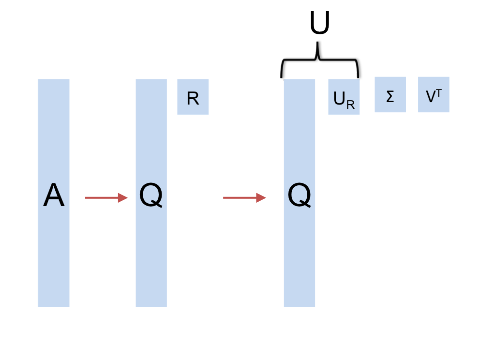
\includegraphics[height=6cm]{ur.png}

Bu demektir ki eğer $R$ üzerinde kütüphanemizin \verb!svd!  çağrısını
kullanırsak (ki $R$ nispeten ufak olduğu için bu ucuz olur) ele geçen $U_R$'i
alıp, $Q$ ile çarparsak, $A$ ayrıştırmasının $U$'şunu elde ederiz! $Q$ ile
çarpım eşle/indirge üzerinden yapılabilir, fakat basit bir çarpım işlemi olduğu
için paralelize edilmesi kolaydır (üstteki mrjob script'inde yaptığımız gibi).

Hadoop icin $A^TA$ [6] yazisi

Kaynaklar

[1] Benson, A., {\em Tall-and-skinny Matrix Computations in MapReduce}

[2] Constantine, P. G., Gleich, D. F. , {\em Tall and Skinny QR factorizations in MapReduce architectures}

[3] Dasgupta, S., Gupta, A., {\em An Elementary Proof of a Theorem of Johnson and Lindenstrauss}

[4] Bayramli, Lineer Cebir, {\em Ders 29}

[5] Bayramli, Lineer Cebir, {\em Matris Çarpımı, Ders 1}

[6] [Lineer Cebir ve Hadoop](https://)

\end{document}
